\subsection{Complete-workload operator comparison}
\label{sec:domain-results}
Table~\ref{tab:domain-main} reports the fixed workloads, including startup, method-owned setup, all query stages, and unresolved requests. Times and p95 values are medians of three complete blocks; coverage requires every requested cutoff resolved. All block values are retained in the artifact.
\begin{table*}[t]\centering\small
\caption{Complete policy-domain workloads at 16 MiB retained-state budget. Total seconds and p95 milliseconds are complete-block medians; resolved coverage requires all three cutoffs. DensePruned shares ViewRank\textquotesingle s polynomial certificate. The separated bottom panel is an independent paired cohort with the same compressed representation for both certificates. Compare costs within a panel; absolute times are not pooled across cohorts.}
\label{tab:domain-main}
\begin{tabular}{lrrrrrr}\toprule
& \multicolumn{3}{c}{HotpotQA, 1,000 questions}&\multicolumn{3}{c}{MuSiQue, 2,417 questions}\\
Method & Total (s)&Resolved (\%)&p95 (ms)&Total (s)&Resolved (\%)&p95 (ms)\\\midrule
ViewRank--Sparse & 116.81 & 99.70 & 250.4 & 108.58 & 98.97 & 165.4\\
ViewRank--DensePruned ($10^{-4}$) & 116.46 & 99.30 & 213.9 & 98.03 & 98.47 & 125.5\\
ViewRank--DensePruned ($10^{-6}$) & 136.16 & 99.80 & 229.0 & 103.77 & 99.01 & 127.3\\
Source lifting, full responses & 200.12 & 99.20 & 371.3 & 311.10 & 98.10 & 481.8\\
Native rank-one + source lifting & 215.77 & 99.20 & 369.1 & 340.62 & 98.10 & 479.2\\
\midrule
\multicolumn{7}{l}{\emph{Separate paired cohort A: same compressed representation}}\\
ViewRank--Sparse (paired A) & 129.00 & 99.70 & 276.4 & 113.24 & 98.97 & 178.8\\
SourceLift, compressed (paired A) & 198.00 & 99.20 & 379.7 & 331.59 & 98.06 & 533.2\\
\bottomrule\end{tabular}\end{table*}
The strongest layout-matched comparison is cohort A. Both methods use sparse $L=512$ retention, 128 current-base preview coordinates, and atom tolerance $10^{-6}$; SourceLift receives subdivision depth four. ViewRank--Sparse lowers complete-workload cost in every paired block: 34.7--35.3\% on HotpotQA and 65.9--66.0\% on MuSiQue. All original requests and unresolved outcomes remain included.
Complete-audit counts are 997 versus 992 on HotpotQA and 2392 versus 2370 on MuSiQue, identical across repetitions. Median all-question p95 values are 276.4 versus 379.7 ms and 178.8 versus 533.2 ms, respectively. The shared-domain certificate therefore improves complete cost, resolution and tail latency after matching compressed retention.
The original main cohort also compares full-response source lifting: the primary reduces complete cost by 40.9--41.6\% on HotpotQA and 64.8--65.1\% on MuSiQue. The atom-free rank-one hybrid remains visible alongside it.
The same certificate supports complementary physical layouts. Sparse retention reduces HotpotQA total cost by 14.2\% relative to same-tolerance DensePruned, while DensePruned gives lower total cost on MuSiQue. The fine full-response layout resolves one additional question on each dataset.
\begin{figure}[t]\centering
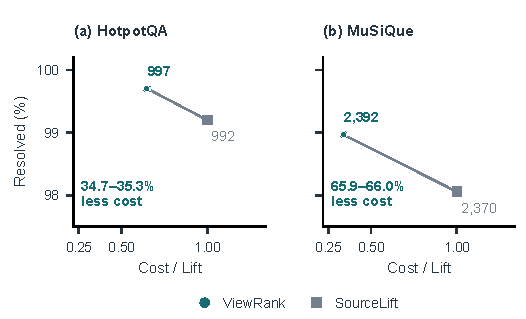
\includegraphics[width=\columnwidth]{../figures/domain_performance.pdf}
\caption{Complete cost and resolution in layout-matched cohort A at 16\,MiB: 1,000/2,417 HotpotQA/MuSiQue questions. Cost is divided by paired compressed SourceLift; all three blocks are plotted and can overlap. Lines join median operating points. Counts require all three cutoffs resolved (\stable\ or verified \unstable); the labeled vertical range magnifies the small coverage differences. All requests, including \unknown, remain charged.}
\label{fig:domain-performance}
\end{figure}
Figure~\ref{fig:domain-performance} places the strongest layout-matched comparison in the cost--resolution plane: ViewRank moves toward lower complete cost and more resolved audits on both workloads. Figure~\ref{fig:domain-coupling} locates the largest active-cost gains in the coupled-source work addressed by the compiler. Table~\ref{tab:domain-main} separately retains the competitive DensePruned layouts and the original full-response controls.

\begin{figure}[t]\centering
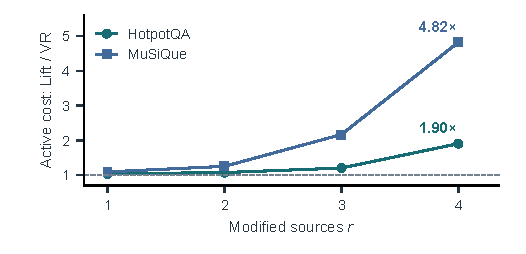
\includegraphics[width=\columnwidth]{../figures/domain_coupling.pdf}
\caption{Source-count strata in cohort A. Lines join medians of three paired ratios of summed active cost; dots retain every block. Every stratum includes \unknown\ requests. Startup/setup are excluded here. Repeated blocks are descriptive, not confidence intervals.}
\label{fig:domain-coupling}\end{figure}

\IfFileExists{generated/domain_source_count.tex}{The $r=1,2,3,4$ strata in Fig.~\ref{fig:domain-coupling} contain 99/232/220/449 original HotpotQA questions and 760/797/253/607 MuSiQue questions. Median SourceLift/ViewRank active-cost ratios are 1.03/1.07/1.20/1.90 and 1.09/1.25/2.17/4.82, respectively. Every stratum and unresolved request remains included; the artifact retains all paired values and counts.
}{}
% Remaining component controls, budgets and fresh-process memory come from their own complete cohorts.
\IfFileExists{generated/domain_supplement_results.tex}{\subsection{Matched mechanism controls}
Table~\ref{tab:domain-ablation} gives a separately scheduled paired block of each complete workload. All methods use the same original questions, policy domain, cutoffs, and 16\,MiB budget. Fixed-precision controls use the primary\textquotesingle s $10^{-6}$ response tolerance. Total costs include every unresolved request; the controller includes both tiers and all retries.
\begin{table}[t]\centering\footnotesize\setlength{\tabcolsep}{2.5pt}
\caption{Matched complete-workload controls, one block per graph. Resolved coverage requires all three cutoffs of a question.}
\label{tab:domain-ablation}
\begin{tabular}{lrrrr}\toprule
&\multicolumn{2}{c}{HotpotQA}&\multicolumn{2}{c}{MuSiQue}\\
Method&Time (s)&Done (\%)&Time (s)&Done (\%)\\\midrule
ViewRank--Sparse & 149.02 & 99.70 & 169.45 & 98.97\\
NoCore & 309.31 & 22.20 & 476.09 & 16.84\\
All-row Scan & 761.84 & 99.80 & 779.80 & 98.97\\
Independent intervals & 143.02 & 46.70 & 140.28 & 52.42\\
Two-tier controller & 138.31 & 99.80 & 199.21 & 99.01\\
\bottomrule\end{tabular}\end{table}
\begin{figure}[t]\centering
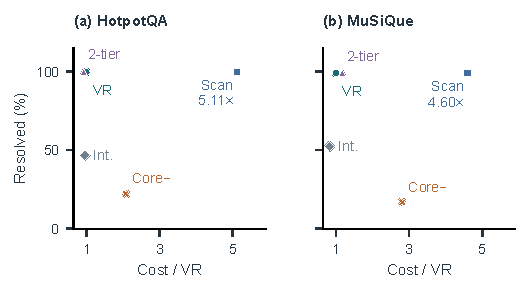
\includegraphics[width=\columnwidth]{../figures/domain_controls.pdf}
\caption{Matched component controls, one complete block per graph. VR: ViewRank; Core$-$: NoCore; Scan: all-row scan; Int.: independent intervals; 2-tier: optional controller. Cost includes all original requests and is normalized to paired VR. Read resolution jointly; Table~\ref{tab:domain-ablation} retains absolute values.}
\label{fig:domain-controls}\end{figure}
Figure~\ref{fig:domain-controls} makes the component effects visible jointly: a cheaper but unresolved workload is distinct from a complete-cost improvement at comparable or better resolution.
All-row Scan costs 5.11$\times$/4.60$\times$ VR on HotpotQA/MuSiQue with nearly identical resolution (Table~\ref{tab:domain-ablation}). NoCore changes both source coherence and its recertified posterior allowance, raising total cost while reducing completion to 222/407 questions. Independent intervals cost 4.0\%/17.2\% less but resolve only 467/1267 questions, so their saving is a cost--coverage tradeoff. The optional controller is 7.2\% faster on HotpotQA and 17.6\% slower on MuSiQue; its p95 rises to 404.3/338.7\,ms from 305.9/234.3\,ms. Fixed fine precision remains the primary.

\subsection{Certificate capacity and process memory}
Figure~\ref{fig:domain-budget} reports separate witness-free certificate-capacity runs: one paired block per graph at each budget. Success requires all three cutoffs STABLE for an original question. Tables~\ref{tab:domain-main} and~\ref{tab:domain-ablation} instead report complete three-valued audit resolution.
\begin{figure}[t]\centering
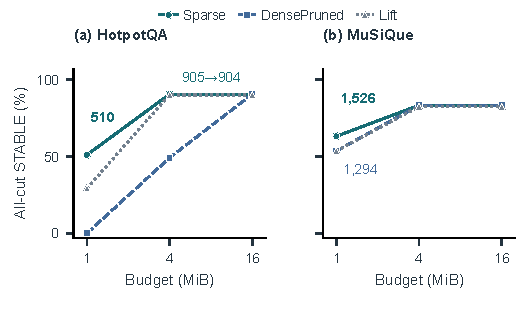
\includegraphics[width=\columnwidth]{../figures/domain_budget.pdf}
\caption{Certificate capacity at 1/4/16\,MiB: Sparse and DensePruned use the same polynomial proof; Lift uses compressed source lifting. Counts label selected points. Every original question remains in the denominator; success requires all three cutoffs \stable. Witness search is uniformly off. One block per setting; admitted numerical state is distinct from process memory.}
\label{fig:domain-budget}\end{figure}
At 1\,MiB, Sparse certifies all cutoffs for 510/1000 versus 0 for DensePruned and 293 for sparse lifting on HotpotQA; the corresponding MuSiQue counts are 1526/2417 versus 1294 for DensePruned and 1296 for sparse lifting.
At 4\,MiB, compressed retention certifies exactly the same 905 HotpotQA and 2014 MuSiQue original questions as fine DensePruned at 16\,MiB. Independent comparison confirms identical question sets and memberships at every cutoff. These are the measured configurations in Fig.~\ref{fig:domain-budget}. The Sparse HotpotQA counts are 905 at 4\,MiB and 904 at 16\,MiB; preview rows depend on cache-miss history and need not be nested across budgets. All attempted work remains charged.
\begin{table}[t]\centering\footnotesize\setlength{\tabcolsep}{2.5pt}
\caption{Fresh single-method processes, one complete run per graph at 16\,MiB with fine responses and no audit serialization. Wall is recorded producer time (seconds); peak is the cumulative process peak working set (MiB) read at block end, including the graph and backend.}
\label{tab:domain-memory}
\begin{tabular}{lrrrr}\toprule
&\multicolumn{2}{c}{HotpotQA}&\multicolumn{2}{c}{MuSiQue}\\
Method&Wall&Peak&Wall&Peak\\\midrule
ViewRank--Sparse & 140.17 & 368.8 & 117.73 & 170.1\\
DensePruned & 162.54 & 424.2 & 110.23 & 179.6\\
SourceLift, compressed & 199.81 & 356.9 & 353.26 & 166.9\\
\bottomrule\end{tabular}\end{table}
Table~\ref{tab:domain-memory} uses fresh single-method processes without audit serialization. Wall spans source freezing through execution, excluding final-summary serialization; cumulative OS working-set peaks include the graph/backend and generation scratch as well as admitted state.
}{}
